\chapter{JT60-SA control design}

\section{Machine description}

JT60-SA is an under-construction superconductive tokamak located at one of the facilities from the National Institutes for Quantum and Radiological Science and Technology (QST)  at  Naka, Japan whose principal purpose is  the contribution to early realization of fusion energy by supporting the exploitation and resolving key physics for ITER reactor. Figure ~\ref{JT60schm} shows the overall general configuration and the most remarkable elements of the machine. The JT-60SA  vacuum chamber will have a major radius of 2.96 m and a minor radius of 1.18 m with an overall plasma volume of 132 $m^3$ ~\cite{Spears2014} .
\smallskip
\begin{figure}
	\centering
	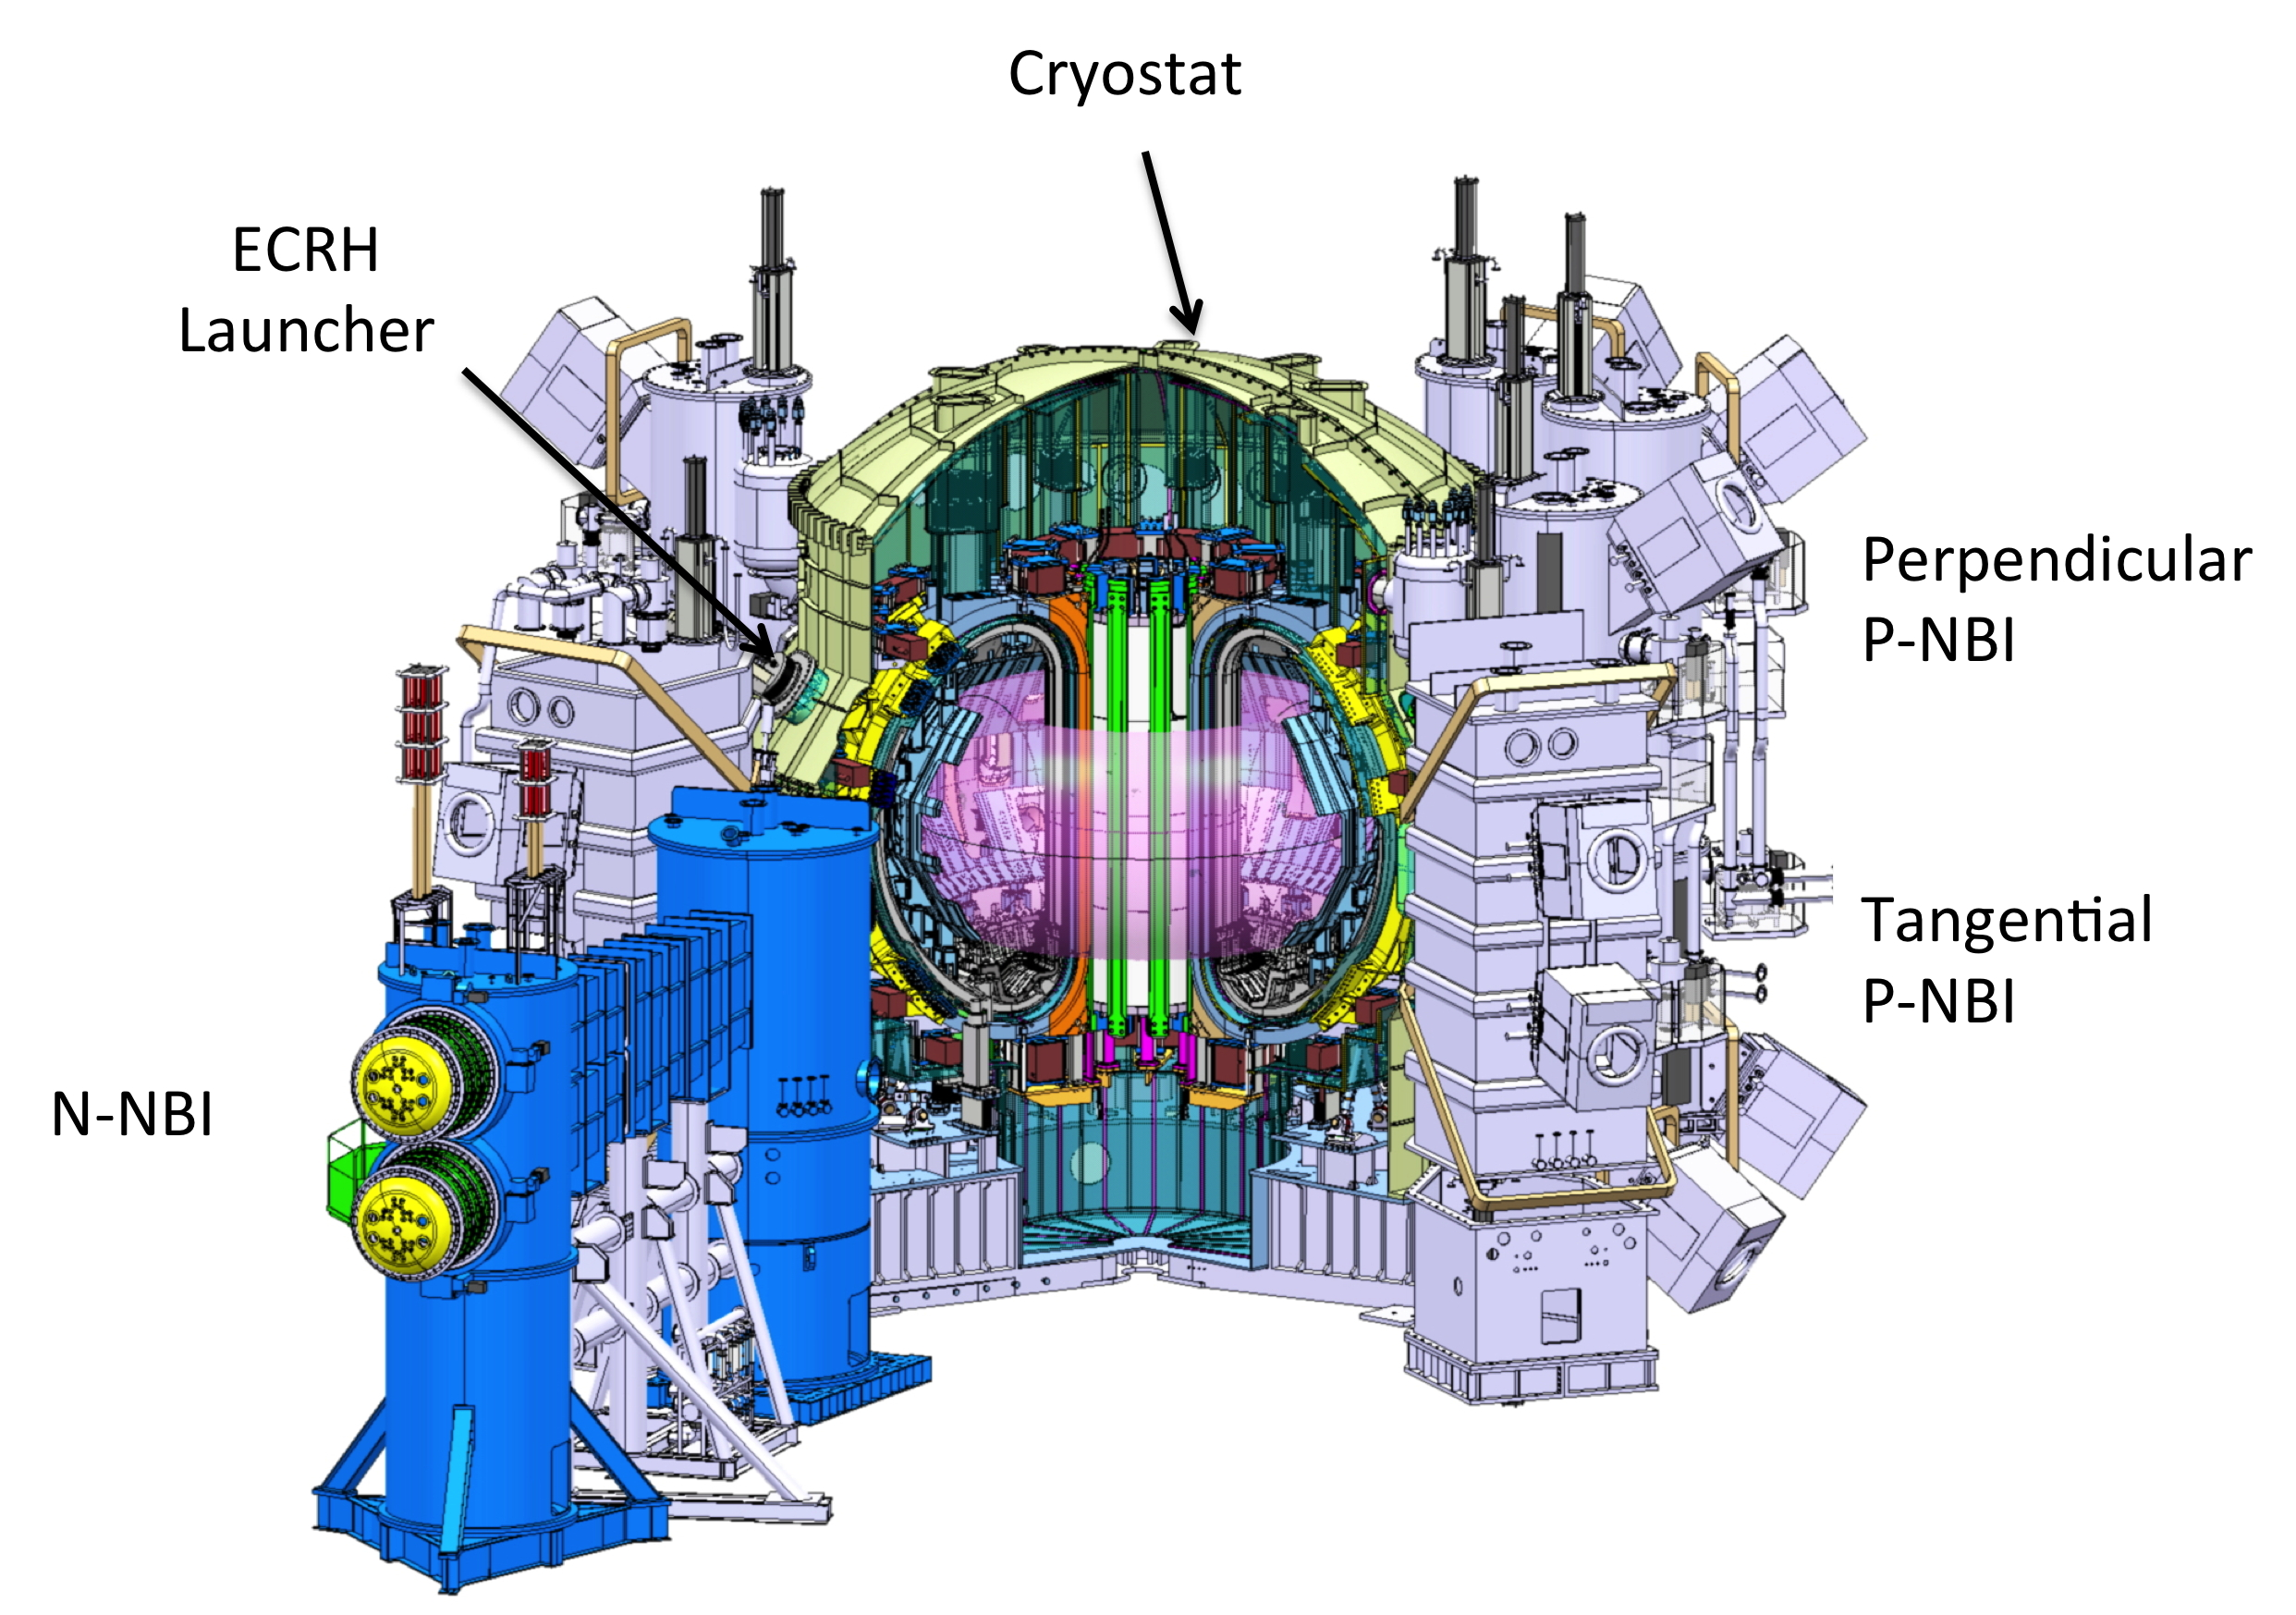
\includegraphics[width=0.80\textwidth]{Chp3/JT60SA.png}
	
	\caption{\label{JT60schm}JT60-SA tokamak configuration ~\cite{JT60SA:ResearchPlan}.}
\end{figure}



The poloidal field coils shown in fig. ~\ref{JT60coils} consist of two sets of superconductive coils: the Equilibrium Field Coils (EF1–6) made

 10 external superconductive coils and 2 in-vessel coils (FPPC1 and FPPC2). 


\begin{figure}
	\centering
	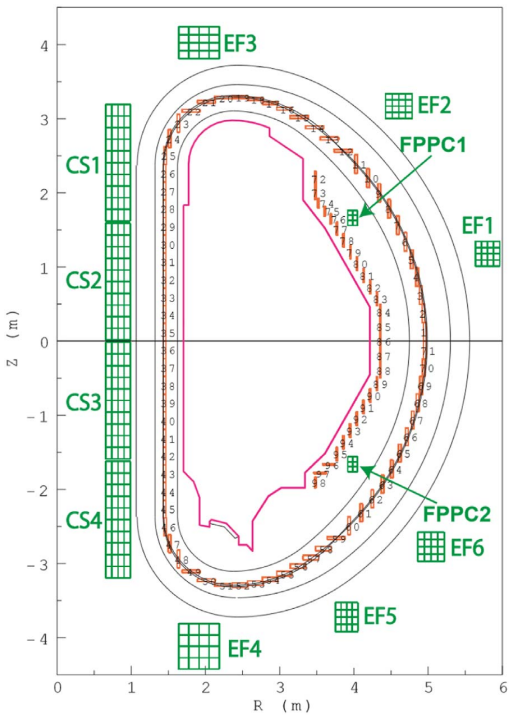
\includegraphics[width=0.6\textwidth]{Chp3/JT60Coils.png}

	\caption{	\label{JT60coils}JT-60SA poloidal cross-section and layout of the Poloidal Field coils system ~\cite{NCruz}.}
\end{figure}


This chapter will address two different approaches for the Last Closed Flux Surface (LCFS) reconstruction an for the  plasma current, shape and position controllers on  JT60-SA in order to achieve and maintain the desired operational scenario given certain equilibrium. 

\section{CREATE magnetic reconstruction tools}
Consorzio di Ricerca per l' Energia, l' Automazione e le Tecnologie dell' Elettromagnetismo (CREATE)

\section{Controller design}
The JET (Joint European Torus) tokamak was the first machine where around 2005 a new model based plasma current and shape controller was set up and tested  with the existing active circuits and control hardware. The novelty controller was the eXtreme Shape Controller (XSC) and its aim was to improve  the performance of the back then present controller to allow the control of extremely shaped plasmas with higher values of elongation and triangularity ~\cite{Albanese2005} . 
 

\section{QST reconstruction and control implementation}

Along with the CREATE tools presented above  for the reconstruction of the LCFS and the XSC for plasma shape control, a reconstruction code and controller provided by the QST team were tested and compared. This section will briefly describe these two methods and its limitations.  

\subsection{Cauchy Condition Surface reconstruction  method }
The QST Cauchy Condition Surface (CCS) method for the reconstruction of the magnetic last closed flux surface calculates controlled variables for plasma position and shape control such as the poloidal magnetic flux at control points on an isoflux scheme  ~\cite{CCS} . The CCS method allows a selection up to 19 geometrical control points and . 

\subsection{QST magnetic controller (FBC)}

~\cite{FBC}

The QST magnetic controller FBC uses the PF coils signals to control the plasma current $I_p$ and the FPPC coils signals for plasma position control.

QST magnetic controller calculates command values of active coil ccurrents/voltages from some information

\begin{equation}
I_{PF\_ref}(t+\Delta t) = I_{PF}(t_0)+M^\dagger_{PF}\left[G_{SP}\delta\Psi_s(t)+G_{SI}\int_{t_0}^{t}\delta\Psi_s(t)dt+G_{XP}\delta\Psi_X(t)+G_{XI}\int_{t0}^{t}\delta\Psi_x(t)dt\right]
\end{equation}

\begin{equation}
V_{com}=G_{vt}\left[M_{coil}\frac{(I_{coil\_ref}-I_{coil\_meas})}{dt}+ \frac{M_{plasma\_now} \cdot I_{p\_now} - M_{plasma\_ bfr} \cdot I_{p\_bfr}}{dt}\right]
\end{equation}

\begin{equation}
I_{FPPC\_ref}(t+\Delta t)=I_{FPPC}(t_0)+ M^\dagger_{FPPC}\left[G_{FP}\delta \Psi_{SF}(t) + G_{FD}\frac{d}{dt}\delta\Psi_{SF}(t) \right]
\end{equation}



\section{Simulation results}	

 The simulations for  the JT60-SA CREATE model ,the XSC, the CCS reconstruction method and the QST controller  were programmed on top of  \textsc{Matlab} and \textsc{Simulink} blocks.
 
 
\begin{figure}
	\centering
	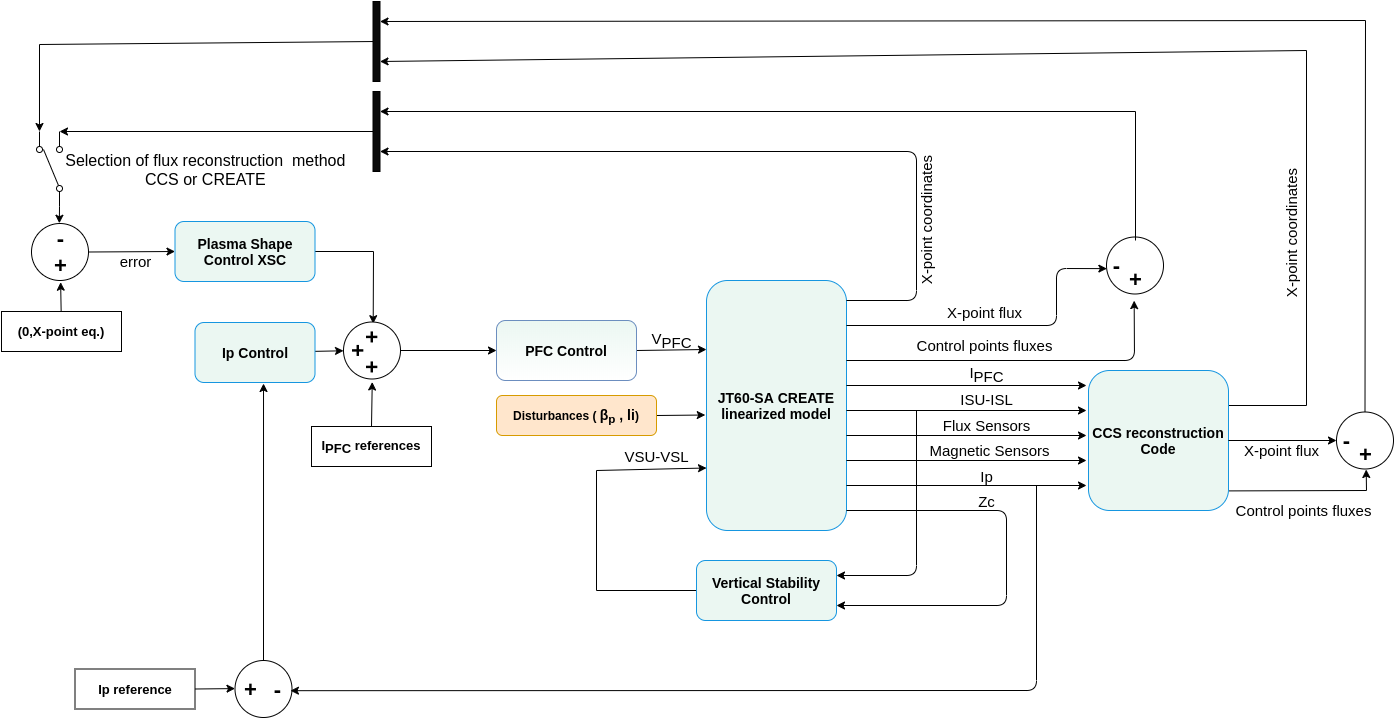
\includegraphics[width=1.05\textwidth]{Chp3/JT60Schemes1.png}
	\caption{	\label{JT60controlscheme}JT-60SA }
\end{figure}

\begin{figure}
	\centering
	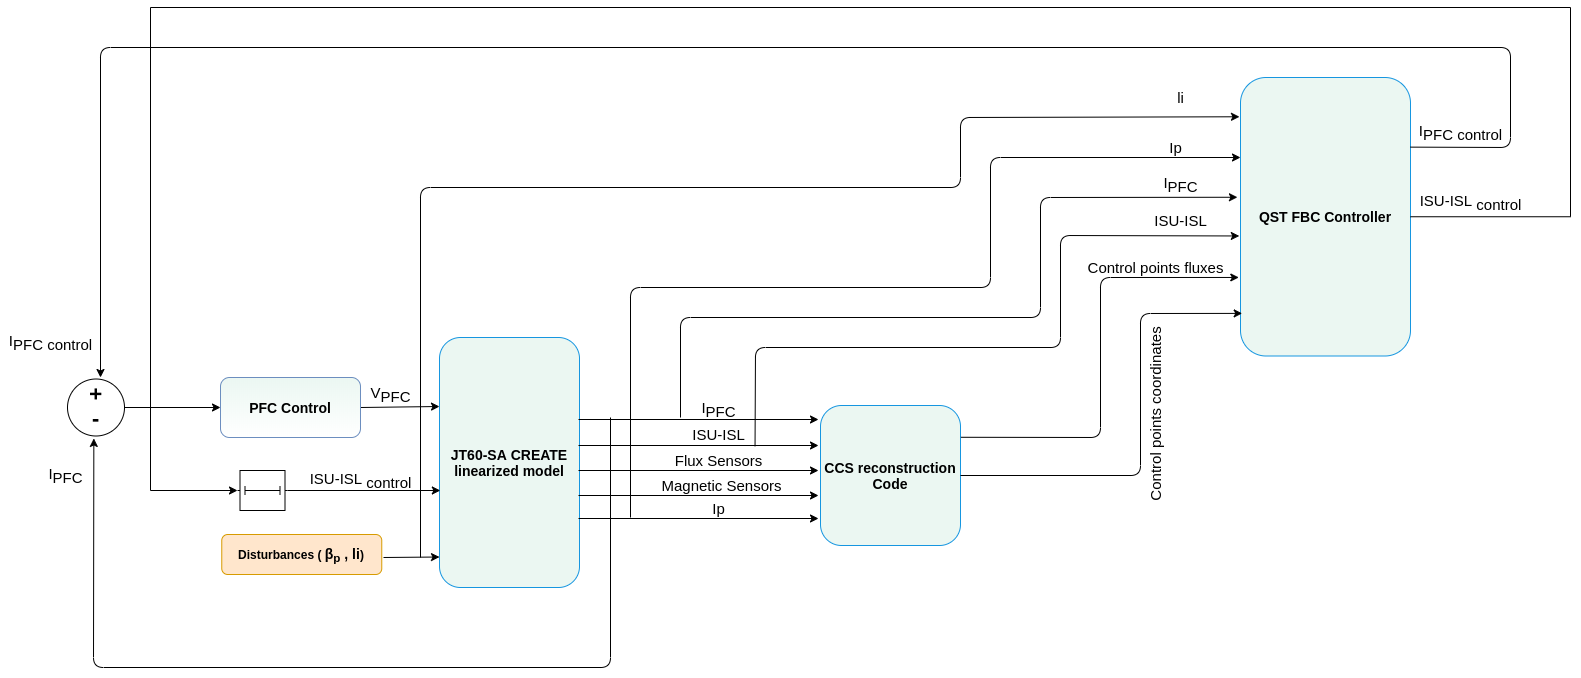
\includegraphics[width=1\textwidth]{Chp3/JT60SchemeFBC.png}
	\caption{	\label{JT60FBCcheme}JT-60SA }
\end{figure}



\subsection{Urano}
\subsection{ELM}
\subsection{Compound ELM}
\subsection{Minor Disruption}

% Please add the following required packages to your document preamble:
% \usepackage[table,xcdraw]{xcolor}
% If you use beamer only pass "xcolor=table" option, i.e. \documentclass[xcolor=table]{beamer}
% Please add the following required packages to your document preamble:
% \usepackage[table,xcdraw]{xcolor}
% If you use beamer only pass "xcolor=table" option, i.e. \documentclass[xcolor=table]{beamer}
\begin{table}[]
	\centering
	\begin{tabular}{|l|c|c|c|c|c|c|}
		\hline
		\rowcolor{color2}
		\multicolumn{7}{|c|}{\textbf{Minor disruption steady state error}}                                                                                                                   \\ \hline
		\rowcolor{color1}
		Controller                                                            & \multicolumn{4}{c|}{eXtreme Shape Controller}          & \multicolumn{2}{l|}{QST Controller}                 \\ \hline
		\rowcolor{color3}
		\begin{tabular}[c]{@{}l@{}}LCFS reconstruction \\ method\end{tabular} & \multicolumn{2}{c|}{CCS} & \multicolumn{2}{c|}{CREATE} & \multicolumn{2}{c|}{CCS}                            \\ \hline
		& Rx mm       & Zx mm      & Rx mm        & Zx mm        & Rx mm                    & Zx mm                    \\ \hline
		6 points                                                              & -4.92           & 20.9          & -3.57            & 28.8            & xxx                        & xxx                        \\ \hline
		8 points                                                              & 17.44           & 21.56          & 17.81            & 29.04            & xxx                        & xxx                        \\ \hline
		19 points                                                             & -5.54           & 16.78          & -4.42           & 24.41            & \cellcolor[HTML]{C0C0C0} & \cellcolor[HTML]{C0C0C0} \\ \hline
	\end{tabular}
\caption{Table }
\end{table}



\subsection{Shape reference change}